\section{Problem Formulation}
\label{problemdefinition}
\subsection{Threat Model}
\label{threatmodel}

\begin{figure}[t]
\setlength{\belowcaptionskip}{-15pt}
\centering
\captionsetup[subfigure]{aboveskip=-0.5pt,belowskip=-5pt}
 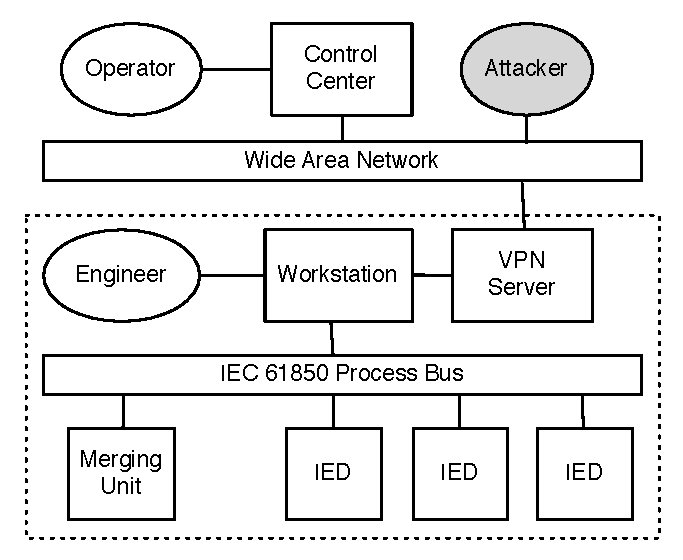
\includegraphics[width=0.6\columnwidth]{figures/substation-outline}
\caption{\scriptsize{A high-level architecture of a smart grid. The dotted area
  represents a substation.}}
 \label{fig:substation}
\end{figure}

One important requirement of a power grid is maintaining
a stable supply of voltage throughout its distribution and transmission
lines. Since many modern grids operate close to their stability
limits, even slight instability or disruption can cause the voltage to
drop below a critical level, forcing load sheddings and in the worst
cast, blackouts. In order to maintain stability, each substation
deploys a number of devices that monitor the voltage level and
dynamically regulate power. A typical high-level architecture of a
smart grid system is shown in Figure~\ref{fig:substation}, with the
dotted box representing one of its substations. A \textit{merging
  unit} collects various analog data from physical sensors (such as
voltage and current levels) and converts them into digital packets,
which are then broadcast over the process bus. A number of intelligent
electronic devices (IEDs), connected to the process bus, look for
anomalous readings in the packets and perform necessary regulating
actions. A \textit{static synchronous compensator} (STATCOM) is one
common type of device for voltage regulation, generating (absorbing)
power when notified of low (high) voltage in the load.

Many modern substations allow engineers to perform maintenance
remotely through a virtual private network (VPN) or other access
mechanisms. While convenient, this also opens up the substation to a
wide range of security attacks, since anyone on the Internet, having
bypassed the VPN, may manipulate various devices through the
workstation.

In this paper, we focus on one particular type of smart grid attacks
and corresponding defense mechanisms, orignally proposed in
\cite{law2012security}.

\noindent\textbf{Attack} We consider scenarios in which the attacker has
successfully gained access to the workstation by exploiting weakness
in its network perimeter (e.g., misconfigured firewall, weak
password/keys). We assume that the attacker wishes to
remain undetected, and so chooses not to perform drastic actions such
as shutting down the entire substation. Finally, we assume that the
attacker is not capable of physically tampering with the substation
components (e.g., tripping transmission lines using circuit breakers).

We focus on one class of attacks where an attacker manipulates the
behavior of a voltage regulator by injecting false voltage data into
the process bus~\cite{law2012security}. From the attacker's point of
view, this attack is particularly appealing since it can be carried
out in a stealthy manner; by injecting a stream of packets with small
deviations from normal voltage, the attacks may remain undetected by
the system until it results in a catastrophic result (i.e., a
blackout), similar to the way Stuxnet~\cite{farwell2011stuxnet} was
carried out.

In particular, given the actual voltage $v$, the attacker constructs a
packet that indicates a voltage value of $kv$, where $k$ is a constant
multiplicative factor. A STATCOM, having received the false
measurement, may unnecessarily inject (possibly causing overvoltage)
or absorb power from the load (under-voltage). When the actual voltage
drops below a certain level, this results in a load shedding enforced
by undervoltage load shedding relay \cite{lefebvre2004undervoltage}.

\noindent\textbf{Defense} One common mitigation against this type of attack
is the use of encryption to ensure the integrity of the
packets. However, relying on encryption as the sole protection
mechanism may not be sufficient for two reasons:
(1) a smart grid system has real-time requirements, with each packet
being sent and processed in a span of milliseconds, and so resources
required to encrypt and decrypt every packet may be too stringent, and
(2) encryption keys are often stored as part of a configuration file,
which may be easy to obtain once the attacker gains the entry to the
workstation. 

% A hardware-based encryption mechanism may address these
% issues, but they are still not common among IEDs, and so we do not
% discuss it in this paper.

Instead, we consider a threshold-based method for detecting bad data
packets \cite{law2012security}. In this method, the IED allocates an
internal variable to keep track of the number of times $I - I_{ref}$
deviates from 0, where $I$ is the current flowing through the current
generator in the IED, and $I_{ref}$ is a fixed reference current. If
this number exceeds some predefined threshold (frequency variable $\tau$) over a certain time
period, then the IED concludes that the
system may be under attack. The intuition behind this detection method
is that $I - I_{ref}$ should remain close to 0 under normal
circumstances, and that even in an unstable environment, should not
vary no more frequently than $\tau$. The best value for $\tau$ for detecting the cyber-attack varies depending on the specific range of the false voltage data injected by the attacker. Thus the challenge for the defender is to determine the right value for $\tau$ to maximize the detection success rate in response to the changes of the attacker's behaviors. We can adopt Markov game model to analyze this kind of strategic interaction between the defender and attacker, which will be described in the next section.
 
\subsection{Markov Games}

A Markov game is played between two players---the \textit{attacker}
and the \textit{defender}---over a possibly infinite sequence of
\textit{rounds}. During each round, both players perform an
\textit{action} that may cause changes to the state of the system with
some probabilities. Each player receives a corresponding payoff after
selecting an action simultaneously. In our case, since the goal of the
attacker is to trigger load shedding through false data injection
attack, the attacker's payoff may be measured by the amount of load
shedding that its action causes to a grid given the action of the
defender. Conversely, the payoff for the defender is the negation of
the amount of load shedding. The Markov game here is
\textit{zero-sum}; that is, the sum of the attacker's and defender's
payoffs is zero.

Formally, a Markov game consists of:
\begin{itemize}
\item $N$: a finite number of players. In our setting, there are two players (defender and attacker), i.e., $N = \{d, a\}$.
\item $A_i$: the action space of each player. $A_d$ and $A_a$ represent the set of defender's and attacker's actions, respectively. 
\item $S$: a finite set of system states. 
\item $Pr$: transition probability function. Given the current state
  $s$ and the joint action $(d, a)$, $Pr(d, a, s, s^\prime)$ returns the probability that the system transits
  from state $s$ to $s^\prime$ when the defender and the attacker perform
  actions $d$ and $a$, respectively.
\item $R_i$: payoff function of the players. Given $s \in S$, $a \in A_a$, and $d \in
  A_d$, $R_d(s, d, a)$ returns the expected payoff of the
  attacker when the joint action $(d, a)$ is performed under state $s$. Since we are
  interested in zero-sum games, the attacker's corresponding payoff $R_a(s, d, a)$ is exactly the negation of $R_d(s, d, a)$, i.e., $R_a(s, d, a) =  - R_d(s, d, a)$.
\end{itemize}

The behaviors of the attacker and defender from
Section~\ref{threatmodel} can be modeled as follows. First, the action
space of the attacker can be defined as
\begin{equation}
A_a = \{ k_1, k_2, ..., k_{N_a} \}
\end{equation}
where $k_1, k_2,...$ are real constants, $N_a$ is the size of $A_a$,
and for some $i \leq N_a$, $k_i$ corresponds to the injection of a
packet that indicates a voltage level of $k_{i}b$ (i.e., falsely
magnifying the voltage reading by a factor of $k_{i}$).

Similarly, the set of the actions that the defender may
perform is defined as:
\begin{equation}
A_d = \{ \tau_1, \tau_2, ..., \tau_{N_d} \}
\end{equation}
where $\tau_1, \tau_2, ...$ are integer constants, $N_d$ is the size
of $A_D$, and for some $j \leq N_d$, $\tau_j$ refers to the
defender deploying the detection method with the threshold of
$\tau_j$ (i.e., the number of times $I - I_{ref}$ is allowed to cross 0). 

A player's \textit{strategy} $\phi$ is a function that given some
state $s$, returns a probability distribution over the set of actions
that the player may perform in $s$.
